\documentclass[conference]{IEEEtran}
\IEEEoverridecommandlockouts

\usepackage{cite}
\usepackage{amsmath,amssymb,amsfonts}
\usepackage{algorithmic}
\usepackage{graphicx}
\usepackage{textcomp}
\usepackage{xcolor}
\usepackage{booktabs}
\usepackage{multirow}
\usepackage{hyperref}

\begin{document}

\title{Appendix: Predictive Modeling Analysis for Cigarette and Marijuana Use\\
\large Supplementary Material for NSDUH 2012 Analysis}

\author{\IEEEauthorblockN{Hasan Alper AYAZ}
\IEEEauthorblockA{\textit{Computer Engineering} \\
\textit{Galatasaray University}\\
Istanbul, Turkey}
}

\maketitle

\begin{abstract}
This appendix presents supplementary predictive modeling analyses for the main NSDUH 2012 study. We developed two logistic regression models to predict lifetime cigarette and marijuana use based on demographic, psychological, and behavioral factors. The marijuana use model achieved excellent performance (AUC = 0.831, Accuracy = 75.4\%), substantially outperforming the cigarette use model (AUC = 0.616, Accuracy = 65.3\%). Key findings include: (1) cigarette use is the strongest predictor of marijuana use (OR = 8.07 for ever vs. never smoked), (2) risk perception shows strong negative associations with use for both substances, (3) mental distress predicts increased odds of use for both substances, and (4) the models can identify high-risk individuals for targeted prevention interventions.
\end{abstract}

\section{Introduction}

This appendix extends the main analysis by developing predictive models for substance use. While the primary study focused on descriptive statistics and hypothesis testing to understand patterns and associations, these logistic regression models allow us to: (1) quantify the independent effects of multiple predictors simultaneously, (2) assess the predictive accuracy of our theoretical model, (3) identify the most important risk factors, and (4) demonstrate the feasibility of using survey data for risk prediction.

Logistic regression is particularly appropriate for this analysis because our outcomes are binary (ever used vs. never used), and the method provides interpretable coefficients (log-odds and odds ratios) that quantify the relationship between predictors and outcomes while controlling for other variables.

\section{Methodology}

\subsection{Model Specification}

We constructed two separate binary logistic regression models:

\textbf{Model 1 - Cigarette Use Prediction:}
\begin{equation}
\log\left(\frac{p_{\text{cig}}}{1-p_{\text{cig}}}\right) = \beta_0 + \beta_1X_1 + \beta_2X_2 + \beta_3X_3 + \beta_4X_4
\end{equation}

where:
\begin{itemize}
    \item $p_{\text{cig}}$ = probability of ever using cigarettes
    \item $X_1$ = Age category (1=12-17, 2=18-25, 3=26-34, 4=35+)
    \item $X_2$ = Gender (1=Male, 2=Female)
    \item $X_3$ = Cigarette risk perception (1=No risk to 4=Great risk)
    \item $X_4$ = Mental distress score (composite, range 3-15)
\end{itemize}

\textbf{Model 2 - Marijuana Use Prediction:}
\begin{equation}
\begin{split}
\log\left(\frac{p_{\text{mj}}}{1-p_{\text{mj}}}\right) = \gamma_0 + \gamma_1X_1 + \gamma_2X_2 + \gamma_3X_3 \\ + \gamma_4X_4 + \gamma_5X_5
\end{split}
\end{equation}

where additional variable:
\begin{itemize}
    \item $X_5$ = Cigarette ever used (0=No, 1=Yes)
\end{itemize}

\subsection{Data Preparation and Sampling}

Cases with missing values on any predictor variable were excluded using listwise deletion. The final analytical samples comprised:
\begin{itemize}
    \item Cigarette model: 37,490 cases (67.8\% of full sample)
    \item Marijuana model: 37,248 cases (67.4\% of full sample)
\end{itemize}

Because the mental distress items were administered only to adults, all respondents aged 12-17 are excluded by listwise deletion. Both models therefore describe adults aged 18 and older, and the age category predictor takes only the values 2-4. As in the main study, the models are unweighted.

We employed an 80-20 train-test split with stratified sampling to ensure that class distributions in training and test sets matched the full dataset. All continuous predictors were standardized (z-score normalization: $z = (x - \mu)/\sigma$) to enable direct comparison of coefficient magnitudes.

Class distributions were: cigarette use (65.2\% users, 34.8\% non-users) and marijuana use (51.0\% users, 49.0\% non-users). The relatively balanced marijuana distribution facilitates unbiased model training.

\subsection{Model Training and Evaluation}

Models were trained using maximum likelihood estimation implemented in scikit-learn's LogisticRegression class with default L2 regularization (C=1.0). Performance was evaluated on the held-out test set using multiple metrics:

\begin{itemize}
    \item \textbf{Accuracy}: Overall proportion of correct predictions
    \item \textbf{Precision}: Proportion of predicted users who are true users (PPV)
    \item \textbf{Recall}: Proportion of true users correctly identified (sensitivity)
    \item \textbf{F1-Score}: Harmonic mean of precision and recall
    \item \textbf{ROC-AUC}: Area under receiver operating characteristic curve
\end{itemize}

\section{Results}

\subsection{Model Performance}

Table \ref{tab:performance} summarizes the performance of both models on the test set.

\begin{table}[htbp]
\centering
\caption{Model Performance on Test Set}
\label{tab:performance}
\begin{tabular}{@{}lrrrrr@{}}
\toprule
\textbf{Model} & \textbf{Acc} & \textbf{Prec} & \textbf{Rec} & \textbf{F1} & \textbf{AUC} \\ \midrule
Cigarette & 0.653 & 0.663 & 0.953 & 0.782 & 0.616 \\
Marijuana & 0.754 & 0.757 & 0.762 & 0.759 & 0.831 \\ \bottomrule
\end{tabular}
\end{table}

The marijuana use model substantially outperformed the cigarette use model across all metrics. The marijuana model achieved excellent discriminatory ability (AUC = 0.831), while the cigarette model showed only moderate performance (AUC = 0.616).

\begin{figure}[htbp]
\centerline{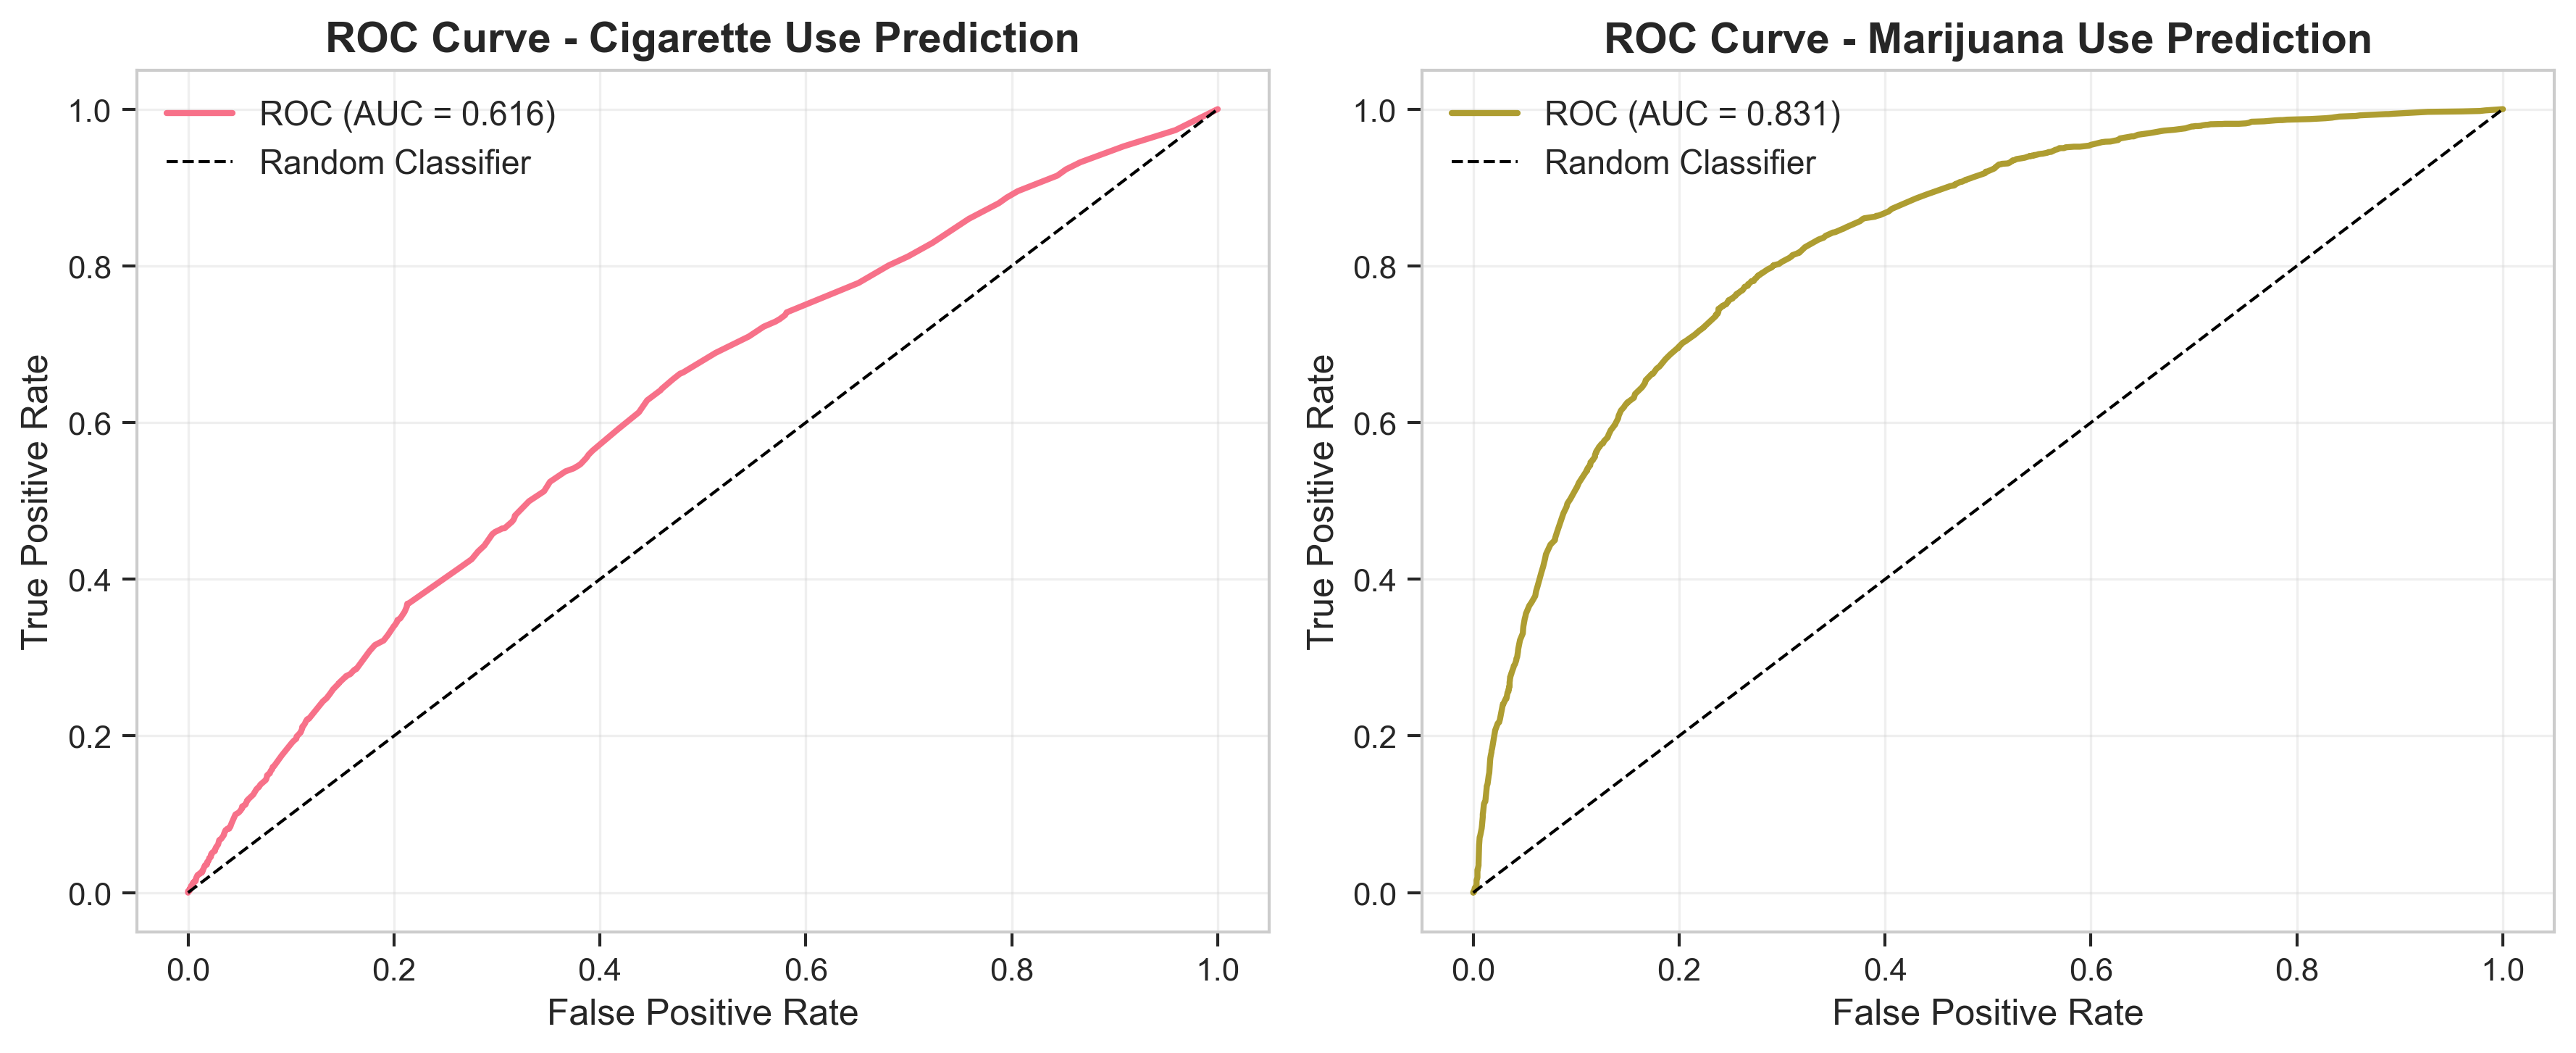
\includegraphics[width=\columnwidth]{figures/fig15_roc_curves.png}}
\caption{ROC curves comparing model performance. The marijuana model (AUC=0.831) shows substantially better discrimination than the cigarette model (AUC=0.616).}
\label{fig:roc}
\end{figure}

Figure \ref{fig:roc} displays the ROC curves for both models. The marijuana curve's substantial separation from the diagonal indicates strong predictive power, while the cigarette curve remains closer to the random classifier line.

\begin{figure}[htbp]
\centerline{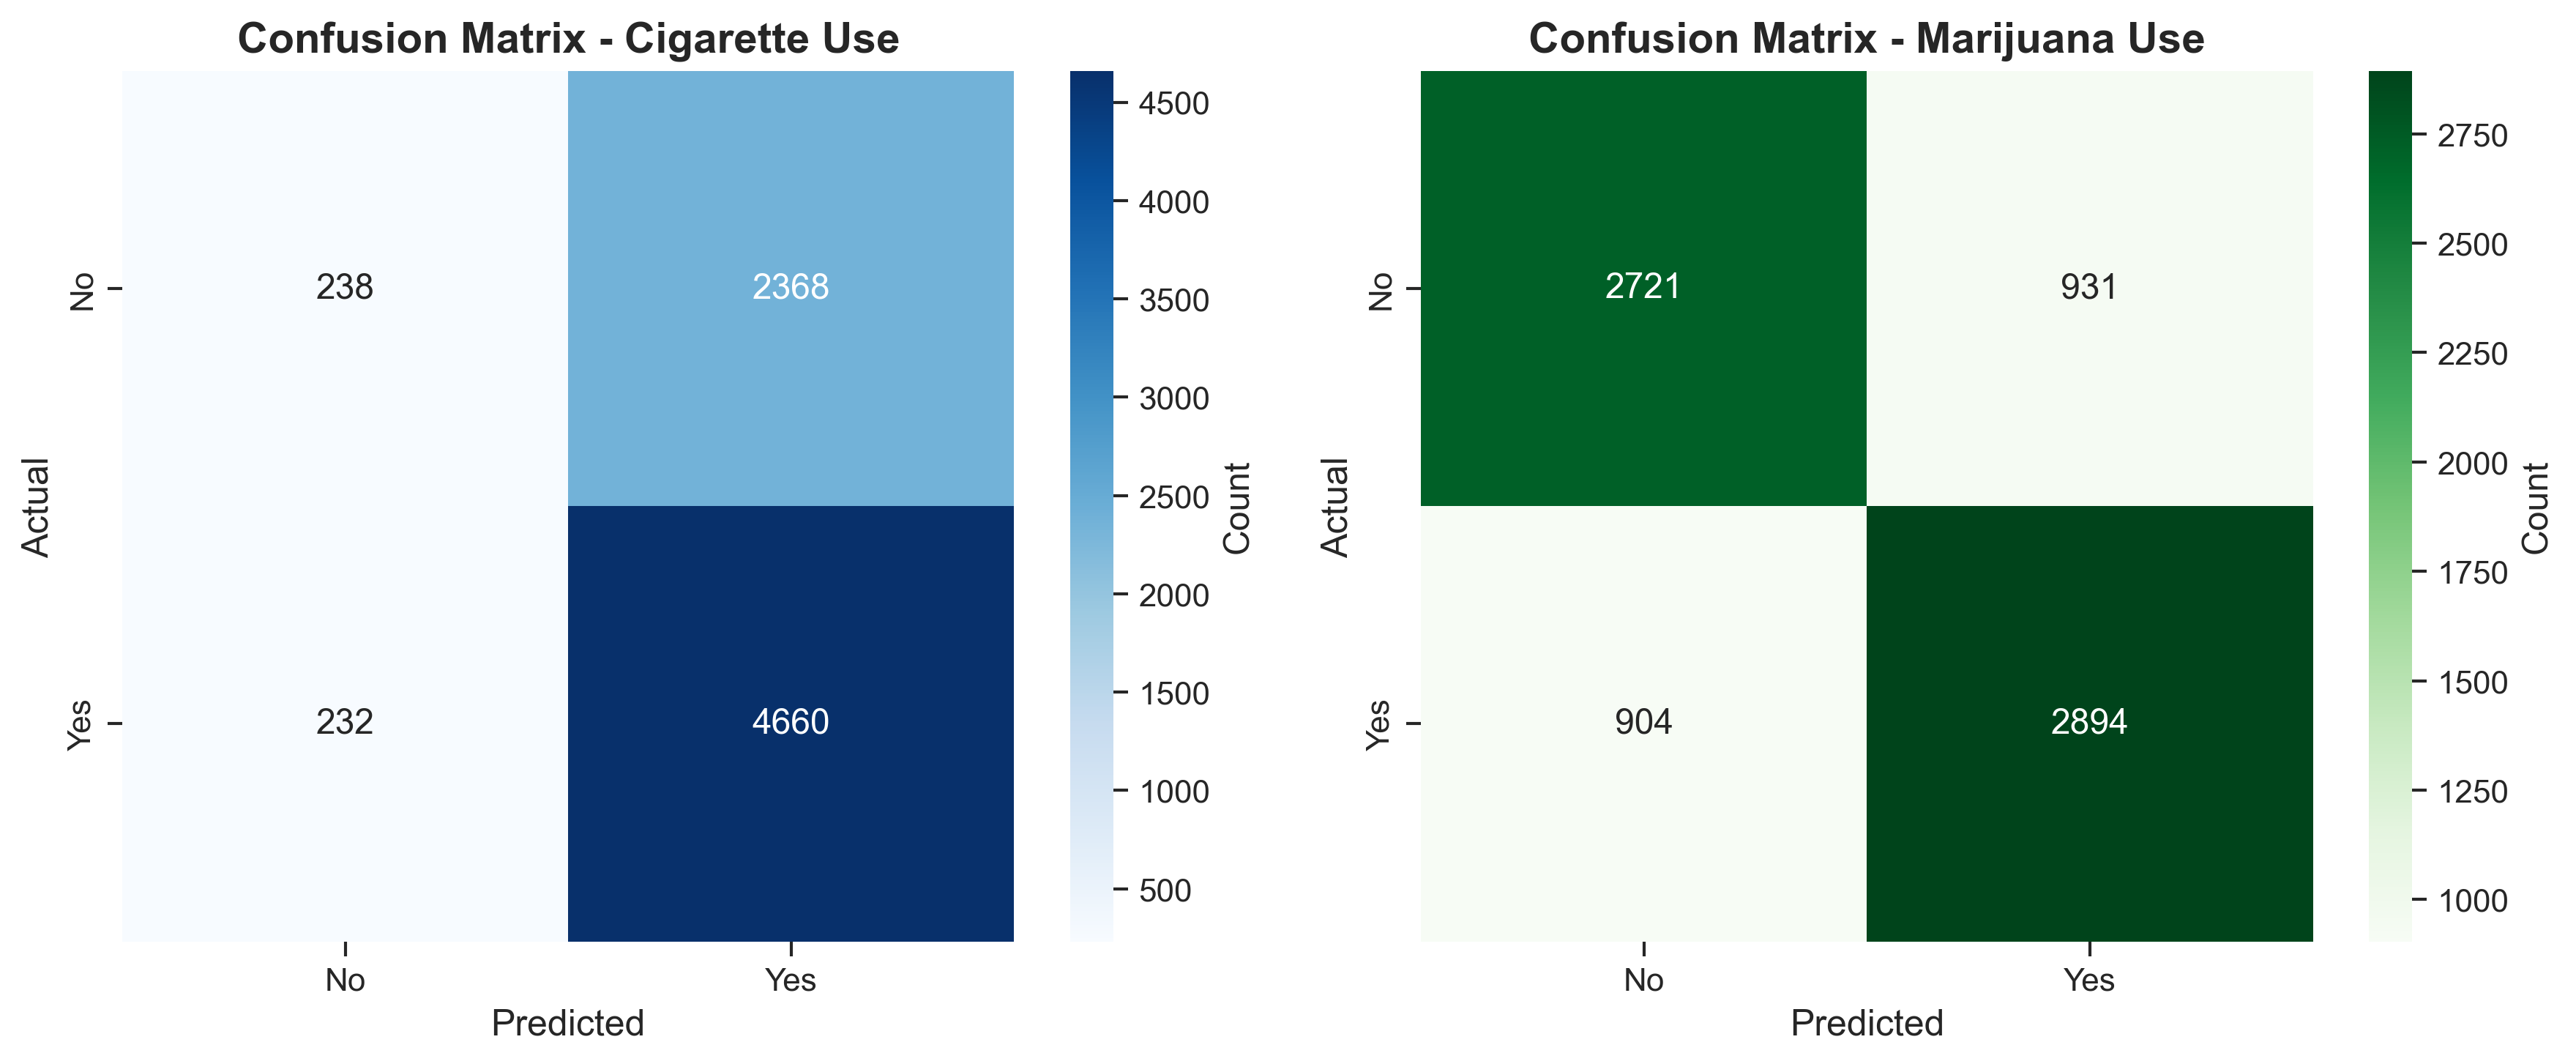
\includegraphics[width=\columnwidth]{figures/fig16_confusion_matrices.png}}
\caption{Confusion matrices showing prediction results on test data.}
\label{fig:confusion}
\end{figure}

The confusion matrices (Figure \ref{fig:confusion}) reveal different error patterns. The cigarette model exhibits high recall (95.3\%) but lower precision (66.3\%), producing many false positives (2,368) but few false negatives (232). This approach identifies most users but also misclassifies many non-users. Since 65.2\% of the sample are users, a trivial classifier that always predicts ``user'' would reach an accuracy of 0.652, so the cigarette model's accuracy (0.653) is essentially no better than this baseline; its AUC of 0.616 shows only weak ranking ability. The marijuana model shows more balanced performance with similar precision and recall.

\subsection{Coefficient Estimates}

Table \ref{tab:coef} presents the standardized coefficients and odds ratios for both models.

\begin{table}[htbp]
\centering
\caption{Logistic Regression Coefficients and Odds Ratios}
\label{tab:coef}
\small
\begin{tabular}{@{}lrrr@{}}
\toprule
\textbf{Predictor} & \textbf{$\beta$ (std.)} & \textbf{OR/SD} & \textbf{OR/unit} \\ \midrule
\multicolumn{4}{l}{\textbf{Cigarette Use Model}} \\ \midrule
Age Category & 0.236 & 1.266 & 1.294 \\
Gender (Female) & -0.206 & 0.814 & 0.662 \\
Cig Risk Perception & -0.208 & 0.813 & 0.745 \\
Mental Distress & 0.247 & 1.280 & 1.106 \\
Intercept & 0.658 & - & - \\ \midrule
\multicolumn{4}{l}{\textbf{Marijuana Use Model}} \\ \midrule
Age Category & -0.004 & 0.996 & 0.996 \\
Gender (Female) & 0.011 & 1.011 & 1.022 \\
MJ Risk Perception & -0.929 & 0.395 & 0.426 \\
Mental Distress & 0.168 & 1.183 & 1.071 \\
Cigarette Ever Used & 0.994 & 2.702 & 8.071 \\
Intercept & 0.013 & - & - \\ \bottomrule
\end{tabular}
\end{table}

All predictors, including the binary ones, were standardized before fitting, so the coefficients and the ``OR/SD'' column refer to a one-standard-deviation change. The ``OR/unit'' column converts each coefficient back to the original scale ($\exp(\beta/\sigma)$): one age category, female vs. male (gender coded 1 = male, 2 = female), one point on the risk scale, one point of distress, and ever vs. never smoked. Because scikit-learn does not report standard errors, the table does not include p-values or confidence intervals.

\subsubsection{Cigarette Use Model Interpretation}

\textbf{Mental Distress} ($\beta$ = 0.247, OR = 1.28): Each standard deviation increase in mental distress (about 2.4 points) is associated with 28\% higher odds of cigarette use, controlling for other factors. This positive association is consistent with theories linking psychological distress to substance use.

\textbf{Age Category} ($\beta$ = 0.236, OR = 1.27): Each standard deviation increase in age category is associated with 27\% higher odds of cigarette use (29\% per category). Because adolescents are not in the model, this reflects differences among adult age groups (18-25, 26-34, 35+), consistent with the descriptive finding that lifetime prevalence is higher in older adult groups.

\textbf{Risk Perception} ($\beta$ = -0.208, OR = 0.81): Higher perceived risk of cigarette smoking is associated with 19\% lower odds of use per standard deviation increase. This effect is modest, suggesting that risk perception alone is insufficient for cigarette prevention.

\textbf{Gender} ($\beta$ = -0.206, OR = 0.81): With gender coded 1 = male and 2 = female, the negative coefficient means that females have lower odds of cigarette use than males. On the original scale, females have about 34\% lower odds than males (OR = 0.66), controlling for age, risk perception, and mental distress.

\subsubsection{Marijuana Use Model Interpretation}

\textbf{Cigarette Ever Used} ($\beta$ = 0.994, OR = 2.70): Because this binary predictor was standardized, the OR of 2.70 refers to one standard deviation. On the original scale, individuals who have smoked cigarettes have about 8.1 times the odds of having used marijuana compared to never-smokers, controlling for the other factors. This is the strongest predictor in either model and quantifies the co-occurrence pattern described in the main study; given the cross-sectional design, it is consistent with, but does not establish, the gateway hypothesis.

\textbf{MJ Risk Perception} ($\beta$ = -0.929, OR = 0.40): This strong negative coefficient indicates that each standard deviation increase in marijuana risk perception is associated with 61\% lower odds of use (57\% lower per point on the 1-4 scale). This is the second-strongest effect and suggests that risk perception is a more powerful determinant of marijuana use than cigarette use.

\textbf{Mental Distress} ($\beta$ = 0.168, OR = 1.18): Mental distress maintains a positive association, with each standard deviation increase linked to 18\% higher odds of marijuana use.

\textbf{Age and Gender}: These variables show minimal effects in the marijuana model when controlling for other factors, suggesting that their bivariate associations with marijuana use are largely mediated by risk perception and cigarette use.

\begin{figure}[htbp]
\centerline{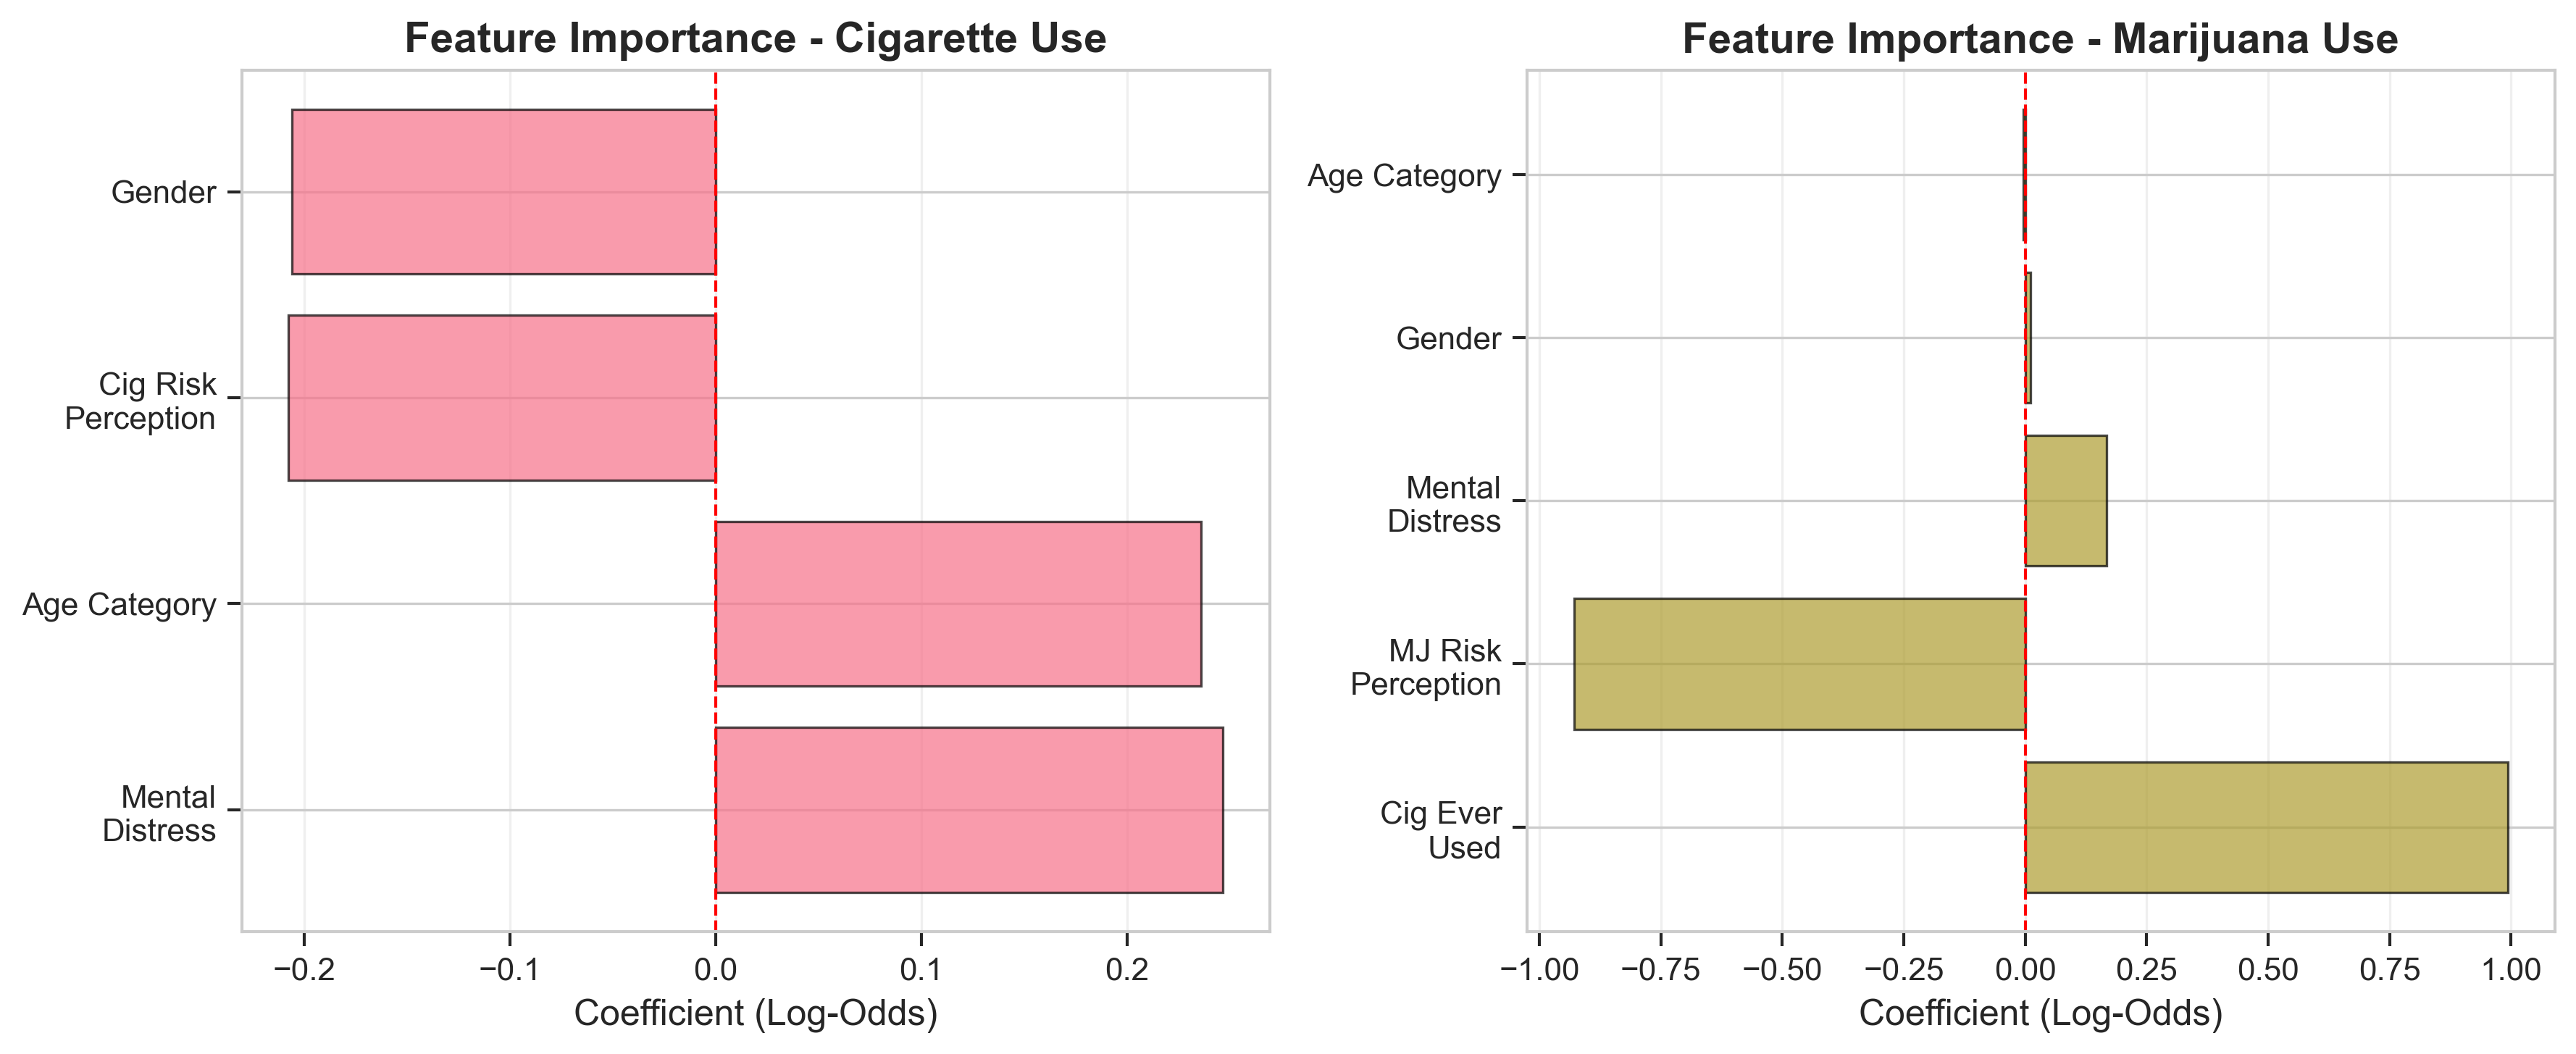
\includegraphics[width=\columnwidth]{figures/fig17_feature_importance.png}}
\caption{Feature importance ranked by absolute coefficient magnitude. Cigarette use and marijuana risk perception dominate the marijuana model, while effects are more evenly distributed in the cigarette model.}
\label{fig:importance}
\end{figure}

Figure \ref{fig:importance} visualizes relative predictor importance. For marijuana use, cigarette use and risk perception clearly dominate, while cigarette use shows more balanced importance across predictors.

\begin{figure}[htbp]
\centerline{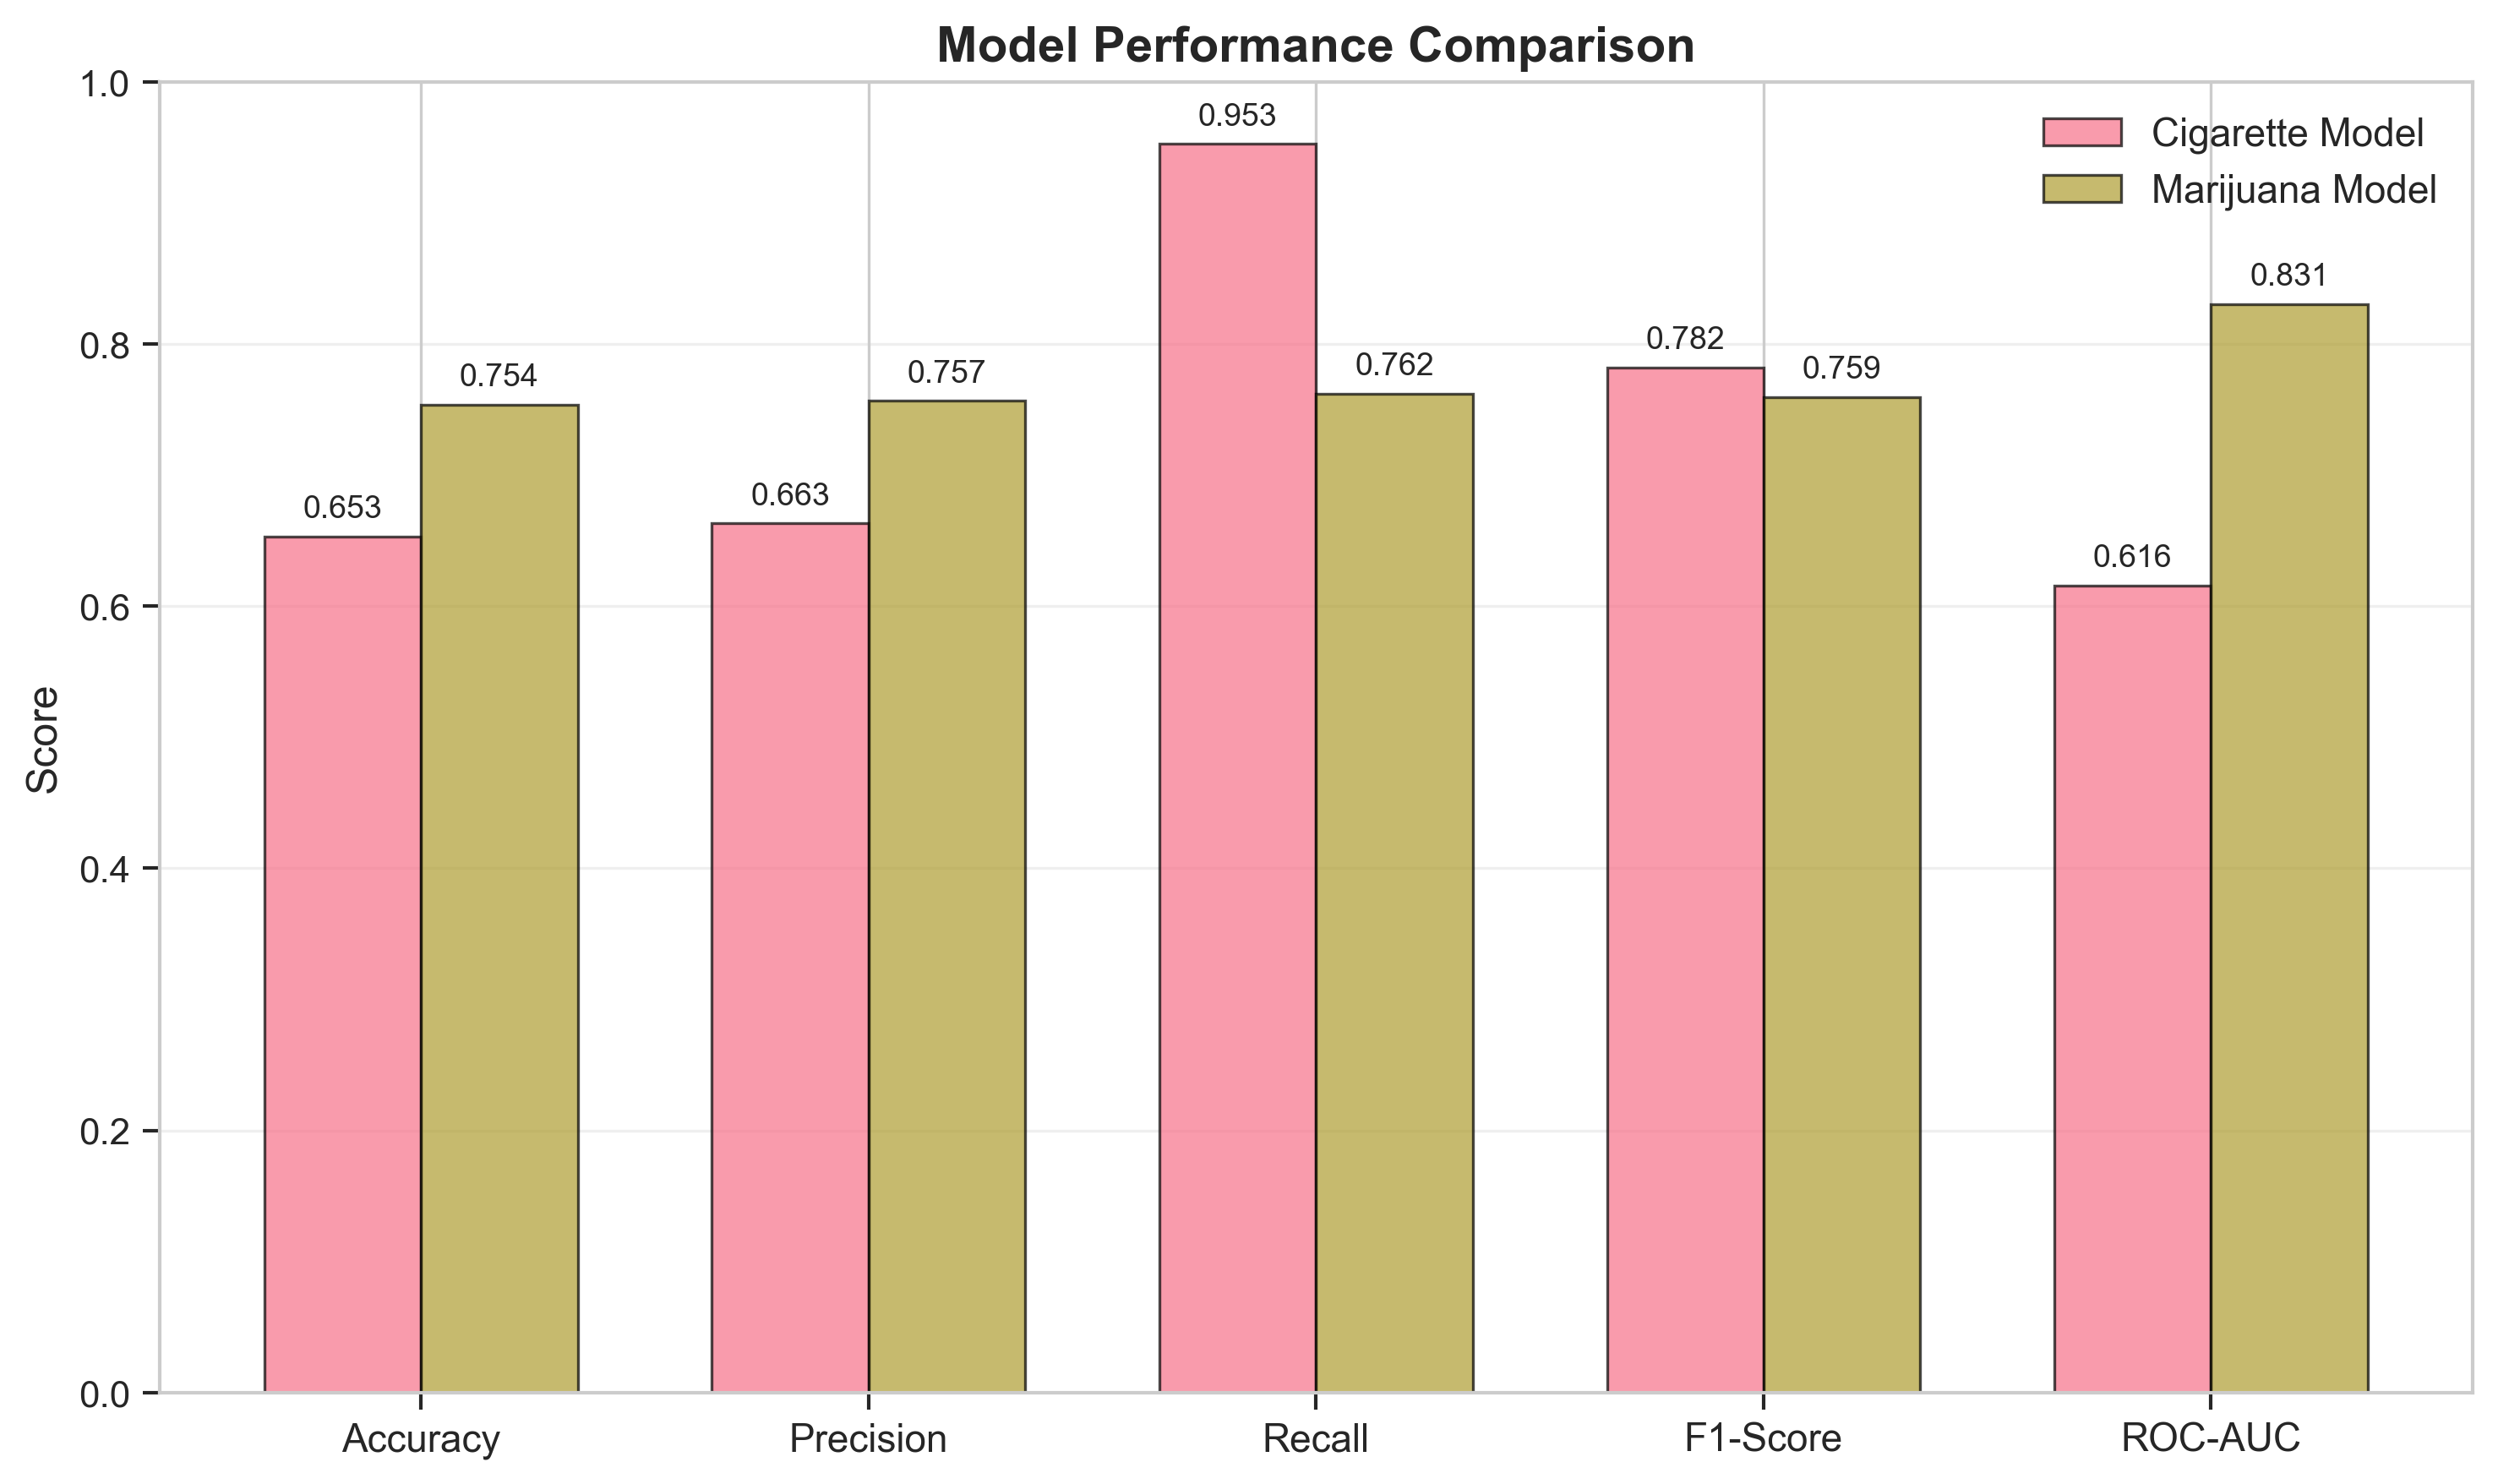
\includegraphics[width=\columnwidth]{figures/fig18_model_comparison.png}}
\caption{Comprehensive comparison of model performance across all evaluation metrics.}
\label{fig:comparison}
\end{figure}

\section{Discussion}

\subsection{Model Performance Comparison}

The substantial performance difference between models (AUC: 0.831 vs. 0.616) can be attributed to several factors:

\textbf{Strong Predictors}: The marijuana model includes cigarette use, which has a very strong association with marijuana use (OR = 8.07 for ever vs. never smoked). Additionally, marijuana risk perception shows much stronger predictive power than cigarette risk perception.

\textbf{Unmeasured Factors}: The cigarette model's moderate performance suggests that important predictors are missing. Factors such as peer smoking, parental smoking, socioeconomic status, and early-life adversity likely play significant roles but are not captured in our model.

\textbf{Outcome Variance}: Marijuana use may be more strongly determined by the measured psychological and behavioral factors, whereas cigarette use may be more influenced by social-environmental factors not included in the model.

\subsection{Implications for Prevention}

These models have practical applications for prevention science:

\textbf{Risk Stratification}: The models can identify high-risk individuals for targeted interventions. For example, adults with high mental distress, low risk perception, and cigarette use represent the highest-risk profile for marijuana use. Extending this to adolescents would require predictors available for that age group.

\textbf{Modifiable Factors}: Both models highlight risk perception as a modifiable target for intervention, particularly for marijuana prevention where the effect is strongest (OR = 0.40).

\textbf{Integrated Approaches}: The strong cigarette-marijuana association (OR = 8.07) supports integrated prevention programs addressing multiple substances rather than siloed approaches.

\textbf{Mental Health Screening}: The consistent association between mental distress and both outcomes underscores the importance of mental health screening in substance use prevention.

\subsection{Limitations}

Several limitations merit consideration:

\begin{itemize}
    \item \textbf{Cross-sectional design}: Cannot establish temporal ordering or causality
    \item \textbf{Lifetime use outcome}: Models predict ever-use rather than current use or problematic use patterns
    \item \textbf{Missing predictors}: Important variables (peer use, family history) not available
    \item \textbf{Sample restriction}: Listwise deletion reduced sample size by $\sim$32\% and removed all respondents aged 12-17
    \item \textbf{No inference}: Unweighted models without standard errors; coefficients describe associations, not significance tests
    \item \textbf{Generalizability}: Models trained on 2012 data may not generalize to current populations
\end{itemize}

\subsection{Future Directions}

Future work could:
\begin{itemize}
    \item Develop models predicting current use, frequency, or dependence
    \item Incorporate additional predictors (peer influence, family history)
    \item Apply machine learning methods (random forests, neural networks)
    \item Validate models on independent datasets
    \item Conduct longitudinal modeling to predict use initiation
    \item Develop age-specific models for targeted prevention
\end{itemize}

\section{Conclusion}

This appendix demonstrates that logistic regression models using demographic, psychological, and behavioral predictors can effectively predict substance use, particularly for marijuana (AUC = 0.831). The models quantify independent effects of risk factors and identify cigarette use (OR = 8.07 for ever vs. never smoked) and risk perception (OR = 0.40 for marijuana) as key predictors. These findings support integrated prevention approaches addressing multiple substances and mental health. While the moderate performance of the cigarette model (AUC = 0.616) indicates missing predictors, both models provide quantitative evidence supporting the main study's conclusions and demonstrate feasibility of predictive modeling using survey data.

\section*{Acknowledgment}

This supplementary analysis was conducted as part of the comprehensive NSDUH 2012 investigation. The author thanks reviewers for suggesting additional predictive modeling analyses to complement the primary descriptive and inferential statistics.

\begin{thebibliography}{00}
\bibitem{hosmer2013} D. W. Hosmer, S. Lemeshow, and R. X. Sturdivant, \textit{Applied Logistic Regression}, 3rd ed. Hoboken, NJ: Wiley, 2013.
\bibitem{james2013} G. James, D. Witten, T. Hastie, and R. Tibshirani, \textit{An Introduction to Statistical Learning}, New York: Springer, 2013.
\bibitem{scikit} F. Pedregosa et al., ``Scikit-learn: Machine Learning in Python,'' \textit{Journal of Machine Learning Research}, vol. 12, pp. 2825-2830, 2011.
\end{thebibliography}

\end{document}